\section{Estimating parameters using \effest}

\subsection{Quick reference}
\label{ss:qeffest}

\begin{verbatim}

usage: effest [-h] [-f ref_fasta] [-i iso_list] [-c nr_cycles] [-m mean_eff]
              [-M max_eff] [-d dist_fam] [-g out_fasta] [-j out_json]
              [-e expr_mul] [-a] [-t] [-w step_size] [-s out_count_file]
              [-k in_count_file] [-p out_prior_file] [-o in_prior_file]
              [-q min_qual] [-r report_file] [-l log_file] [-v]
              [input file]

Estimate GC-dependent fragment amplification efficiencies and fragment size
distribution from paired-end RNA-seq data mapped to transcriptome (version
1.1).

positional arguments:
  input file         Aligned *paired end* reads in SAM format sorted by
                     *name*.

optional arguments:
  -h, --help         show this help message and exit
  -f ref_fasta       Reference fasta.
  -i iso_list        List of single isoform transcripts.
  -c nr_cycles       Number of PCR cycles (11).
  -m mean_eff        Assumed pool efficiency (0.87).
  -M max_eff         Assumed maximum efficiency (None).
  -d dist_fam        Distribution to model fragment size distribution
                     (n|sn|*auto*).
  -g out_fasta       Output fasta.
  -j out_json        File to store estimated raw parameters (raw_params.json).
  -e expr_mul        Expression level multiplier (10000.0).
  -a                 Do not use GC efficiency correction on expression levels
                     (False).
  -t                 Trim off old expression values (True).
  -w step_size       Sliding window size / step size ratio (5).
  -s out_count_file  Pickle counts to the specified file (effest_counts.pk).
  -k in_count_file   Load counts from specifies file.
  -p out_prior_file  Pickle fragment prior to the specified file
                     (effest_pr.pk).
  -o in_prior_file   Load fragment prior from the specified pickle file.
  -q min_qual        Minimum mapping quality (0).
  -r report_file     Report PDF (effest_report.pdf).
  -l log_file        Log file.
  -v                 Toggle verbose mode (False).

\end{verbatim}

\subsection{Background}


\subsubsection{Scope and limitations}

The implicit simulation model implemented in \rlsim was designed in order to be more complex than the models used for inference
in order to provide the means for fair benchmarking, hence the joint inference of all parameters would not be practical under this model.
However, the most likely use case of an RNA-seq library simulator is to simulate datasets which reproduce the properties of real datasets. For that reason, the \rlsim package provides \effest, a tool to estimate \emph{some} parameters using \texttt{ad-hoc} procedures.

\effest provides an estimate of the empirical fragment size distribution, GC-dependent amplification efficiencies based on a default or user-provided mean amplification efficiency, \emph{relative} expression levels. It does not provide any estimate of length-dependent amplification efficiencies as inferring those would be hard from data generated by standard RNA-seq experiments.

\warn{The estimates provided by \effest are based on naive assumptions as they ignore the interactions between the different experimental factors. However, they are good starting parameters when trying to replicate the properties of a given dataset.}

The \effest tool is implemented in \texttt{Python}, relying on the \texttt{HTSeq}, \texttt{NumPy} and related packages.

\subsubsection{Estimating the fragment size distribution}

The fragment size distribution is analysed in the following steps:
\begin{itemize}
    \item The empirical fragment size distribution is estimated by simply normalising the fragment counts in each length category.
    \item The truncated normal and skew normal distributions are fitted to the empirical distribution using a maximum likelihood procedure.
    \item The best fitting analytical distribution is then selected using the Akaike information criterion (AIC) \cite{aic}.
\end{itemize}

The empirical distribution is reported in the raw parameters JSON file, while the best fitting analytical distribution is reported as a part of the suggested \rlsim command line.

\subsubsection{Estimating GC-dependent amplification efficiencies}

Before discussing the details of how \effest estimates the GC-dependent efficiencies from a single paired-end RNA-seq dataset, we first present the theory behind estimating these parameters in the case of ideal custom experiments. This is necessary in order to illustrate the limitations imposed by a single standard dataset and to understand the motivation behind the procedures used by the tool in order to circumvent these limitations.

\paragraph{Idealised PCR experiment with measurable counts}

The figure below illustrates a PCR experiment where we can measure the fragment counts exactly:

\begin{center}
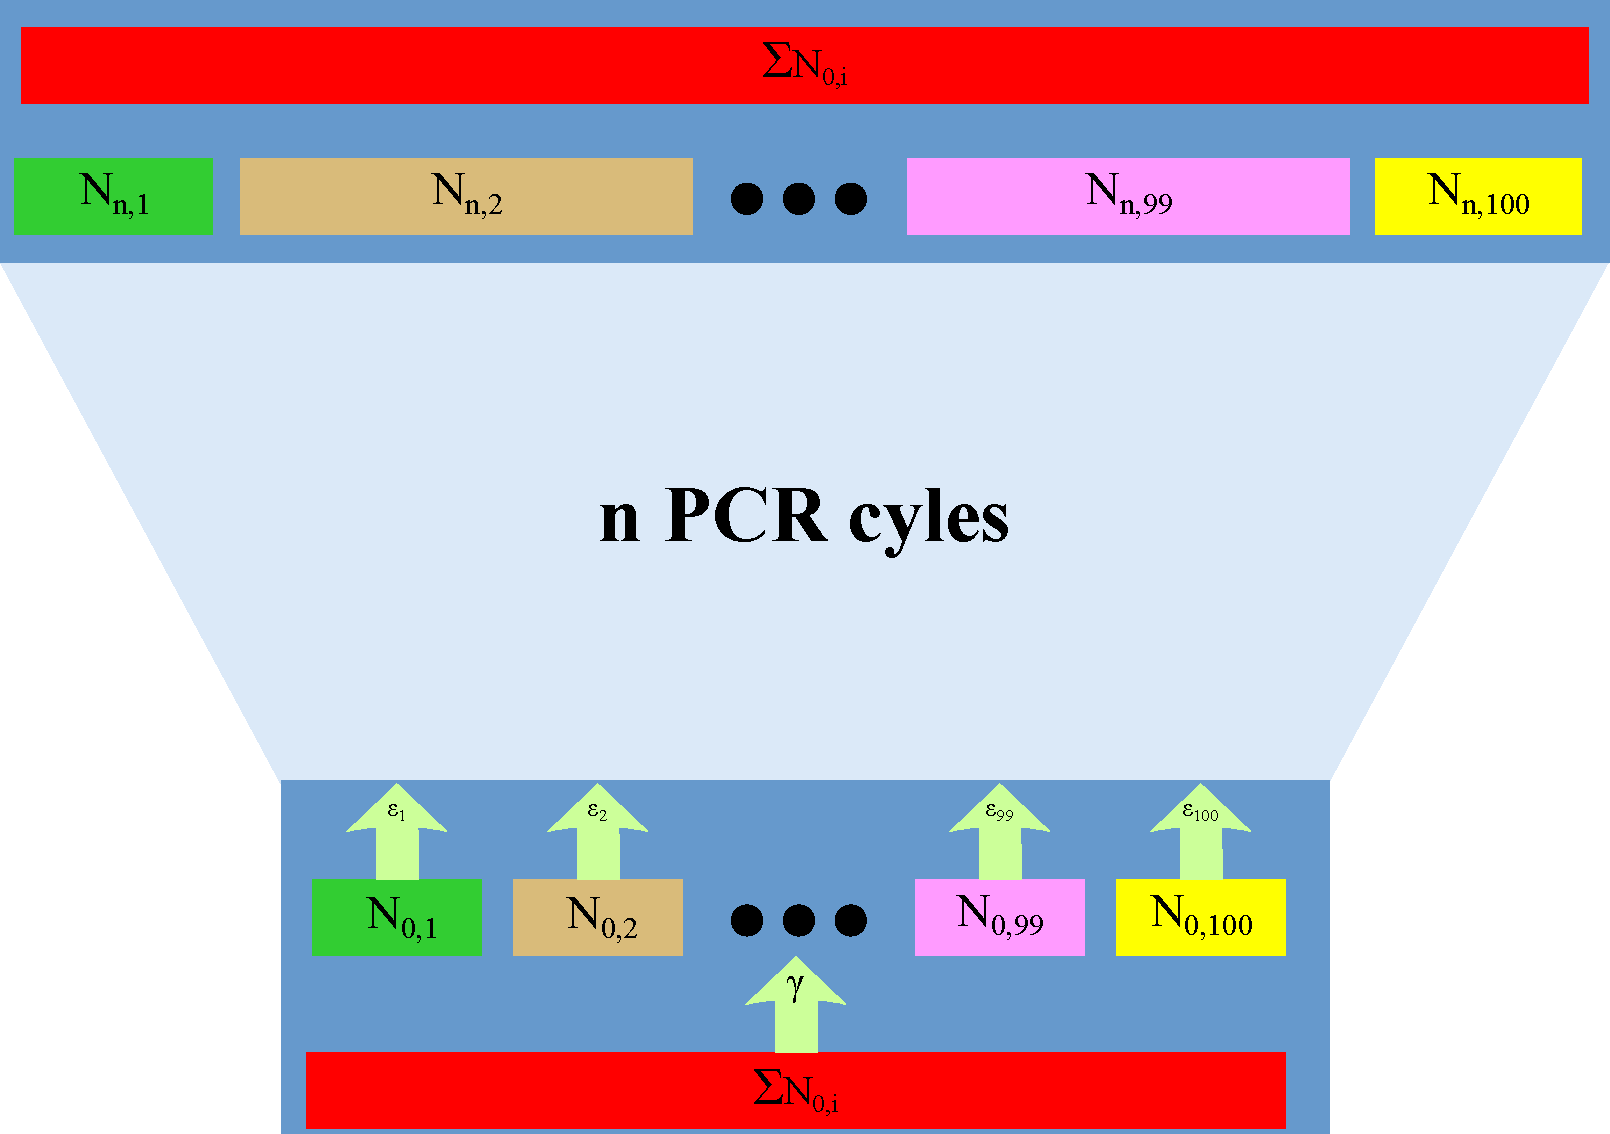
\includegraphics[scale=0.36]{pix/pcr_model.pdf}
\end{center}

The fragments are binned in 100 GC-content bins, $N_{i,j}$ being the number of fragments in the $j^{\mathrm{th}}$ GC content bin during the $i^{\mathrm{th}}$ cycle (e.g. $N_{0,50}$ is the number of fragments with 50\% GC content before PCR amplification). Each GC content bin has an associated amplification efficiency $\epsilon_i$.

PCR amplification on the level of individual bins is modelled as a Galton-Watson \cite{GaltonWatson} branching process with constant efficiencies across cycles, so the expected number of fragments after $n$ cycles in a given bin can be calculated as:

\begin{equation}\label{eq:amp_bin}
    E[N_{n,i}] = N_{0,i}(1+\epsilon_i)^n
\end{equation}

In an idealised PCR experiment where we can measure the fragment \emph{counts} in  individual bins after cycles $n_1$ and $n_2$ the estimation of the amplification efficiencies ($\epsilon_i$) would be trivial. However, RNA-seq experiments allow only for the measurement of \emph{proportions}, hence it is necessary to consider the total number of fragments after $n$ cycles.

\paragraph{Serial measurements of fragment proportions and known pool efficiency}

In order to account for the increase in the size of the fragment pool, we define a Galton-Watson process which acts on all of the fragments (the ``fragment pool'') with a ``pool efficiency'' $\gamma$ satisfying the following equation:

\begin{equation}
    \left(\sum{N_{0,i}}\right) ( 1 + \gamma)^n = \sum{\left[N_{0,1} ( 1 + \epsilon_i)^n\right]}
\end{equation}

Note that despite the fact that $\gamma$ cannot be expressed as a simple linear combination of the individual efficiencies, it is always possible to find a value satisfying the equation above. 

For now, assume that $\gamma$ is know, necessarily obtained from a measurement independent from the fragment proportions calculated from RNA-seq data.
Then the number of fragments in the whole pool after $n$ cycles can be calculated as:

\begin{equation}\label{eq:amp_pool}
    E[\sum N_{n,i}] = \left(\sum N_{0,i}\right) (1+\gamma)^n
\end{equation}

Following equations \ref{eq:amp_bin} and \ref{eq:amp_pool} the \emph{proportion} of the fragments from the $j^{\mathrm{th}}$ bin relative to the whole fragment pool after $n$ PCR cycles can be calculated as:

\begin{equation}
    \pi_{n,j} = \frac{N_{0,j} {(1 + \epsilon_j)}^n}{(\sum_kN_{0,k}) {(1 + \gamma)^n}}
\end{equation}

Then the ratio of proportions after $n_2$ and $n_1$ cycles is:

\begin{equation}
    \frac{\pi_{n_2,j}}{\pi_{n_1,j}} = \frac{{(1+\epsilon_j)}^{n_2 - n_1}}{{(1+\gamma)}^{n_2 - n_1}}
\end{equation}

By rearranging the equation above, we get an expression which can be used for estimating amplification efficiencies:

\begin{equation}\label{eq:eff_est}
    \hat{\epsilon}_j = \exp\left[\frac{1}{n_2 - n_1} \ln\left(\frac{\pi_{n_2,j}}{\pi_{n_1,j}}\right)\right] (1 + \gamma) - 1
\end{equation}

For some bins the ratio of proportions will be necessarily less then one, in which case we set the amplification efficiency to 0 or some arbitrary value.

\paragraph{The pool amplification efficiency ($\gamma$)}

In standard RNA-seq datasets there is no information about the pool amplification efficiency ($\gamma$), so this has to be specified by the user. \emph{In principle}, it should be possible to measure the ``average'' amplification efficiency of the fragment pool using quantitative PCR methods.
The pool efficiency can be directly set via the \texttt{-m} flag, alternatively the user can specify the assumed maximum amplification efficiency through the \texttt{-M} flag.

The default is a pool efficiency (\texttt{-m}) of 0.87, in line with the amplification efficiencies reported in the quantitative PCR literature for individual amplicons \cite{weiss97,karlen07,ruijter09}


\paragraph{Inferring efficiencies from a single dataset}

Standard RNA-seq protocols usually sample the fragments from the amplified fragment pool only after a specified PCR cycle $n_1$, hence there is only a single set of fragment proportion ($\pi_{n_1,j}$) available. At the first glance this should make it impossible to estimate GC-dependent efficiencies using the formulas above. In order to circumvent this problem, \effest employs an \textit{ad-hoc} procedure based on the assumption that the coverage biases are local and hence in the case of long transcripts they ``average out'' without affecting too much the estimates of per-transcript relative expression levels.

If the assumption above hold, we can calculate a ``\textbf{fragment prior}'', reflecting the proportions in the GC content bins if there were no biases present ($\pi_{0,j}$) using the following procedure:

\begin{itemize}
    \item Estimate the fragment size distribution as described above.
    \item For every length category, do a sliding window analysis over a list of specified transcripts. Tabulate the GC content weighted by the relative expression level of the respective transcript and the probability of a fragment having the respective length. Step size used during the sliding window analysis is calculated as the ratio of the fragment size and the value of the \texttt{-w} flag (10 by default).
    \item From the counts resulting from the sliding window procedure, calculate the expected marginal GC content distribution under the assumption of no PCR biases, which is used as proxy for the proportions in the GC content bins before amplification ($\pi_{0,j}$).
\end{itemize}

The amplification efficiencies then are calculated using equation \ref{eq:eff_est} based on the proportions calculated from the data ($\pi_{n_1,j}$), the fragment prior ($\pi_{0,j}$) and the pool efficiency specified by the user ($\gamma$).

\warn{Note that the approach for estimating GC-dependent amplification efficiencies above is rather naive as it ignores the interactions of amplification biases with priming biases and seize selection and it is based on a strong assumption of locality of coverage biases. However, simulations suggest that if the assumption hold, the approach performs well in recovering efficiencies.}

\paragraph{Fitting the GC efficiency function}

After the GC-dependent amplification efficiencies have been estimated as described above, \effest attempts to fit the GC efficiency function
used in \rlsim (equation \ref{eq:gc_eff}). The maximum efficiency is set directly as the observed maximum value, while the minimum efficiency and the shape parameter is obtained by a least squares procedure using the weights $\epsilon_j  (1 - \epsilon_j)$. The weight reflects the fact that usually most of the fragments in real experiments do not have extreme GC contents, hence we expect more reliable data around 50\% of GC content.

The estimated parameters are reported as part of the suggested \rlsim command line parameters.

\subsubsection{Estimating relative expression levels}

The counts of the fragments mapped to a given transcript $t$ are binned by GC content and stored after parsing in a count vector $C_t$.
Then, based on the estimated GC-dependent efficiencies, an ``efficiency weight'' vector ($w$) is calculated for each GC content bin, based on the expected number of descendants of a single molecule from the bin after $n$ PCR cycles:

\begin{equation}
    w_i = \frac{1}{\left(1+\epsilon_i\right)^n}
\end{equation}

The relative expression level of the transcript ($E_t$) is calculated by summing the count vector normalised by the length of the transcript ($l_t$) and the efficiency weight vector and also multiplied by a value supplied by the user through the \texttt{-e} flag ($E_u$):

\begin{equation}
    E_t = \left( \sum_{i=0}^{100} C_{t,i} \frac{w_i}{\mathrm{min}(w)} \right) \frac{1}{l_t} E_u
\end{equation}

Note that the GC-dependent efficiency correction through $w_i$ gives more weight to fragments with lower efficiencies.

The calculated relative expression level is analogous to the widely used FPKM metric, but corrected for the effects of GC-dependent efficiencies.

If the \texttt{-a} flag is specified, \effest will also save uncorrected (``flat'') expression levels in a separate fasta file with the \texttt{flat\_} prefix.
The uncorrected expression levels are multiplied with a constant ($\kappa$) in order to make their overall magnitude similar to the corrected levels:

\begin{equation}
    E_t^f = \left( \sum_{i=0}^{100} C_{t,i} \kappa \right) \frac{1}{l_t} E_u
\end{equation}


As it is impossible to estimate absolute expression levels from standard RNA-seq data, the estimates provided by the above approach can be too high or too small for a particular simulation setting. Hence, the purpose of the $E_u$ multiplier specified through the \texttt{-e} flag ($10^5$ by default) is to globally adjust the expression levels. Using the pickle files generated by \effest as input (see section \ref{sec:pickle}) makes it feasible to tune the relative expression levels, by skipping the parsing of the input data and the generation of fragment prior, which are the most time-consuming steps.

\warn{Always examine carefully the distribution of relative expression levels and expression levels of individual transcripts in order to make sure that they are suitable for you particular simulation setting!}

\subsection{Running the program}

\begin{verbatim}
usage: effest [-h] [-f ref_fasta] [-i iso_list] [-c nr_cycles] [-m mean_eff]
              [-M max_eff] [-d dist_fam] [-g out_fasta] [-j out_json]
              [-e expr_mul] [-a] [-t] [-w step_size] [-s out_count_file]
              [-k in_count_file] [-p out_prior_file] [-o in_prior_file]
              [-q min_qual] [-r report_file] [-l log_file] [-v]
              [input file]

Estimate GC-dependent fragment amplification efficiencies and fragment size
distribution from paired-end RNA-seq data mapped to transcriptome (version
1.1).

positional arguments:
  input file         Aligned *paired end* reads in SAM format sorted by
                     *name*.
\end{verbatim}

\subsubsection{Input files}

The input data is \textbf{name-sorted paired-end} reads in SAM format, mapped to the reference transcriptome
specified via the \texttt{-f} flag.

The file containing the list of single-isoform transcripts (one name per file) is specified through the \texttt{-i} flag. If no file is specified, the full set of transcripts is used for calculation of the fragment size distribution and GC-dependent efficiencies.


\subsubsection{Command line arguments}

\begin{itemize}
    \item[\texttt{-h}]{Show help message and exit.}
    \item[\texttt{-f}]{Reference transcriptome in fasta format (required, no default)}
    \item[\texttt{-i}]{The list of single isoform transcripts used for estimating GC-dependent amplification efficiencies and fragment size distribution (no default).}
    \item[\texttt{-c}]{Number of PCR cycles used in calculations (default: 11).}
    \item[\texttt{-m}]{The assumed pool efficiency ($\gamma$, default: 0.87)}
    \item[\texttt{-M}]{The efficiency assumed for the bin with the highest increase in proportion. Overrides the \texttt{-m} flag when specified.}
    \item[\texttt{-d}]{Distribution family to be fitted on the empirical distribution of fragment sizes. The possible values are \texttt{n} for truncated normal, \texttt{sn} for skew normal and \texttt{auto} for selecting the best fitting family using AIC (default).}
    \item[\texttt{-g}]{The name of the output fasta file, augmented with relative expression levels (default: <input\_name>\_expr.fas).}
    \item[\texttt{-j}]{JSON file to store estimated raw parameters (default: \texttt{raw\_params.json}).}
    \item[\texttt{-e}]{The value of the expression level multiplier ($E_u$, default: $10^4$)}
    \item[\texttt{-a}]{Disable GC-dependent efficiency correction (False).}
    \item[\texttt{-t}]{Do not trim off old expression values from input transcriptome.}
    \item[\texttt{-w}]{Sliding window step size parameter. Step size used for the sliding window analysis is equal to the fragment size divided by the value of this flag (10 by default). Set it to smaller value in order to speed up the calculating of the fragment prior.}
    \item[\texttt{-s}]{The name of the fragment count pickle file (default: \texttt{effest\_counts.pk}).}
    \item[\texttt{-k}]{Use the fragment counts pickled in the specified file as input (no default).}
    \item[\texttt{-p}]{Pickle fragment prior to the specifies file (default: \texttt{effest\_pr.pk}).}
    \item[\texttt{-o}]{Load fragment prior from the specified pickle file (no default).}
    \item[\texttt{-q}]{Minimum mapping quality. Fragment having either reads a mapping quality lower than this value are discarded (default: 0)}
    \item[\texttt{-r}]{Name of the report PDF file (default: \texttt{effest\_report.pdf}).}
    \item[\texttt{-l}]{Name of the log file (default: stderr).}
    \item[\texttt{-v}]{Toggle verbose mode.}
\end{itemize}

\subsubsection{Output files}

\begin{itemize}
    \item{The suggested rlsim parameters are reported to the standard output:
        \begin{verbatim}
Suggested rlsim parameters:
-d "1.0:sn:(364, 132, 2.80662, 190, 925)"
-eg "(4.95603, 0.518537, 1)"
-n 1880365
        \end{verbatim}
    \item{The relative expression levels are reported in the fasta file \texttt{<input\_name>\_expr.fas}, the estimated ``raw'' parameters are saved in a JSON file.}
    \item{The report file contains the following plots:
        \begin{itemize}
            \item the marginal GC content distribution
            \item the marginal fragment size distribution
            \item the joint GC content/fragment size distribution
            \item the ``fragment prior``
            \item the ``marginal GC content prior''
            \item a plot of the estimated GC-dependent efficiencies along with the fitted efficiency function
            \item the distribution of estimated relative expression levels (also with the zero value excluded)
            \item the plots of the truncated normal and skew normal distributions fitted to the fragment size distribution
        \end{itemize}
    }
    }

\end{itemize}
\subsection{Re-using pickles of parsed data}
\label{sec:pickle}

Instead of parsing again the SAM file (which is quite time consuming), \effest allows for using the counts pickle file generated during parsing. Specifying the matching reference transcript file is still necessary:
\begin{verbatim}
    ./effest -v -f test/ref.fas -k test/effest_counts.pk
\end{verbatim}

Using also a pickled fragment prior generated by a previous run makes the analysis fast, which facilitates reanalysis with different parameters:
\begin{verbatim}
    ./effest -v -f test/ref.fas -k test/effest_counts.pk -o effest_pr.pk
\end{verbatim}


